
\documentclass{article}

%
%Margin - 1 inch on all sides
%
\usepackage[letterpaper]{geometry}
\usepackage{times}
\geometry{top=1.0in, bottom=1.0in, left=1.0in, right=1.0in}

%
%Doublespacing
%
\usepackage{setspace}
\doublespacing

%
%Rotating tables (e.g. sideways when too long)
%
\usepackage{rotating}

%
% Indent the first paragraph after section title
%
\usepackage{indentfirst}

%
%allow counting superscript
%
\usepackage[super]{nth}

% use roman numerals for section and subsection
\renewcommand{\thesection}{\Roman{section}} 
\renewcommand{\thesubsection}{\thesection.\Roman{subsection}}

% allow images
\usepackage{graphicx}

% set size of section title
\usepackage{titlesec}
\titleformat*{\section}{\normalfont\bfseries}

%
%Fancy-header package to modify header/page numbering (insert last name)
%
\usepackage{fancyhdr}
\pagestyle{fancy}
\lhead{} 
\chead{} 
\rhead{Last Name \thepage} 
\lfoot{} 
\cfoot{} 
\rfoot{} 
\renewcommand{\headrulewidth}{0pt} 
\renewcommand{\footrulewidth}{0pt} 
%To make sure we actually have header 0.5in away from top edge
%12pt is one-sixth of an inch. Subtract this from 0.5in to get headsep value
\setlength\headsep{0.333in}

%
%Works cited environment
%(to start, use \begin{workscited...}, each entry preceded by \bibent)
% - from Ryan Alcock's MLA style file
%
\newcommand{\bibent}{\noindent \hangindent 40pt}
\newcommand{\annotent}{\medskip \newline}
\newenvironment{workscited}{\newpage \begin{center} Works Cited \end{center}}{\newpage }
\newenvironment{annotation}{\begin{center} Annotated Bibliography \end{center}}{\newpage }

%
%Begin document
%
\begin{document}
\begin{flushleft}

% IMPORTANT!!
%%%%First page name, class, etc
Name \\
Instructor \\
Course \\
Date \\

\begin{center}
    \textbf{TITLE}
\end{center}

%%%%Changes paragraph indentation to 0.5in
\setlength{\parindent}{0.5in}
%%%%Begin body of paper here
\newpage
Picture Example
\begin{figure}
    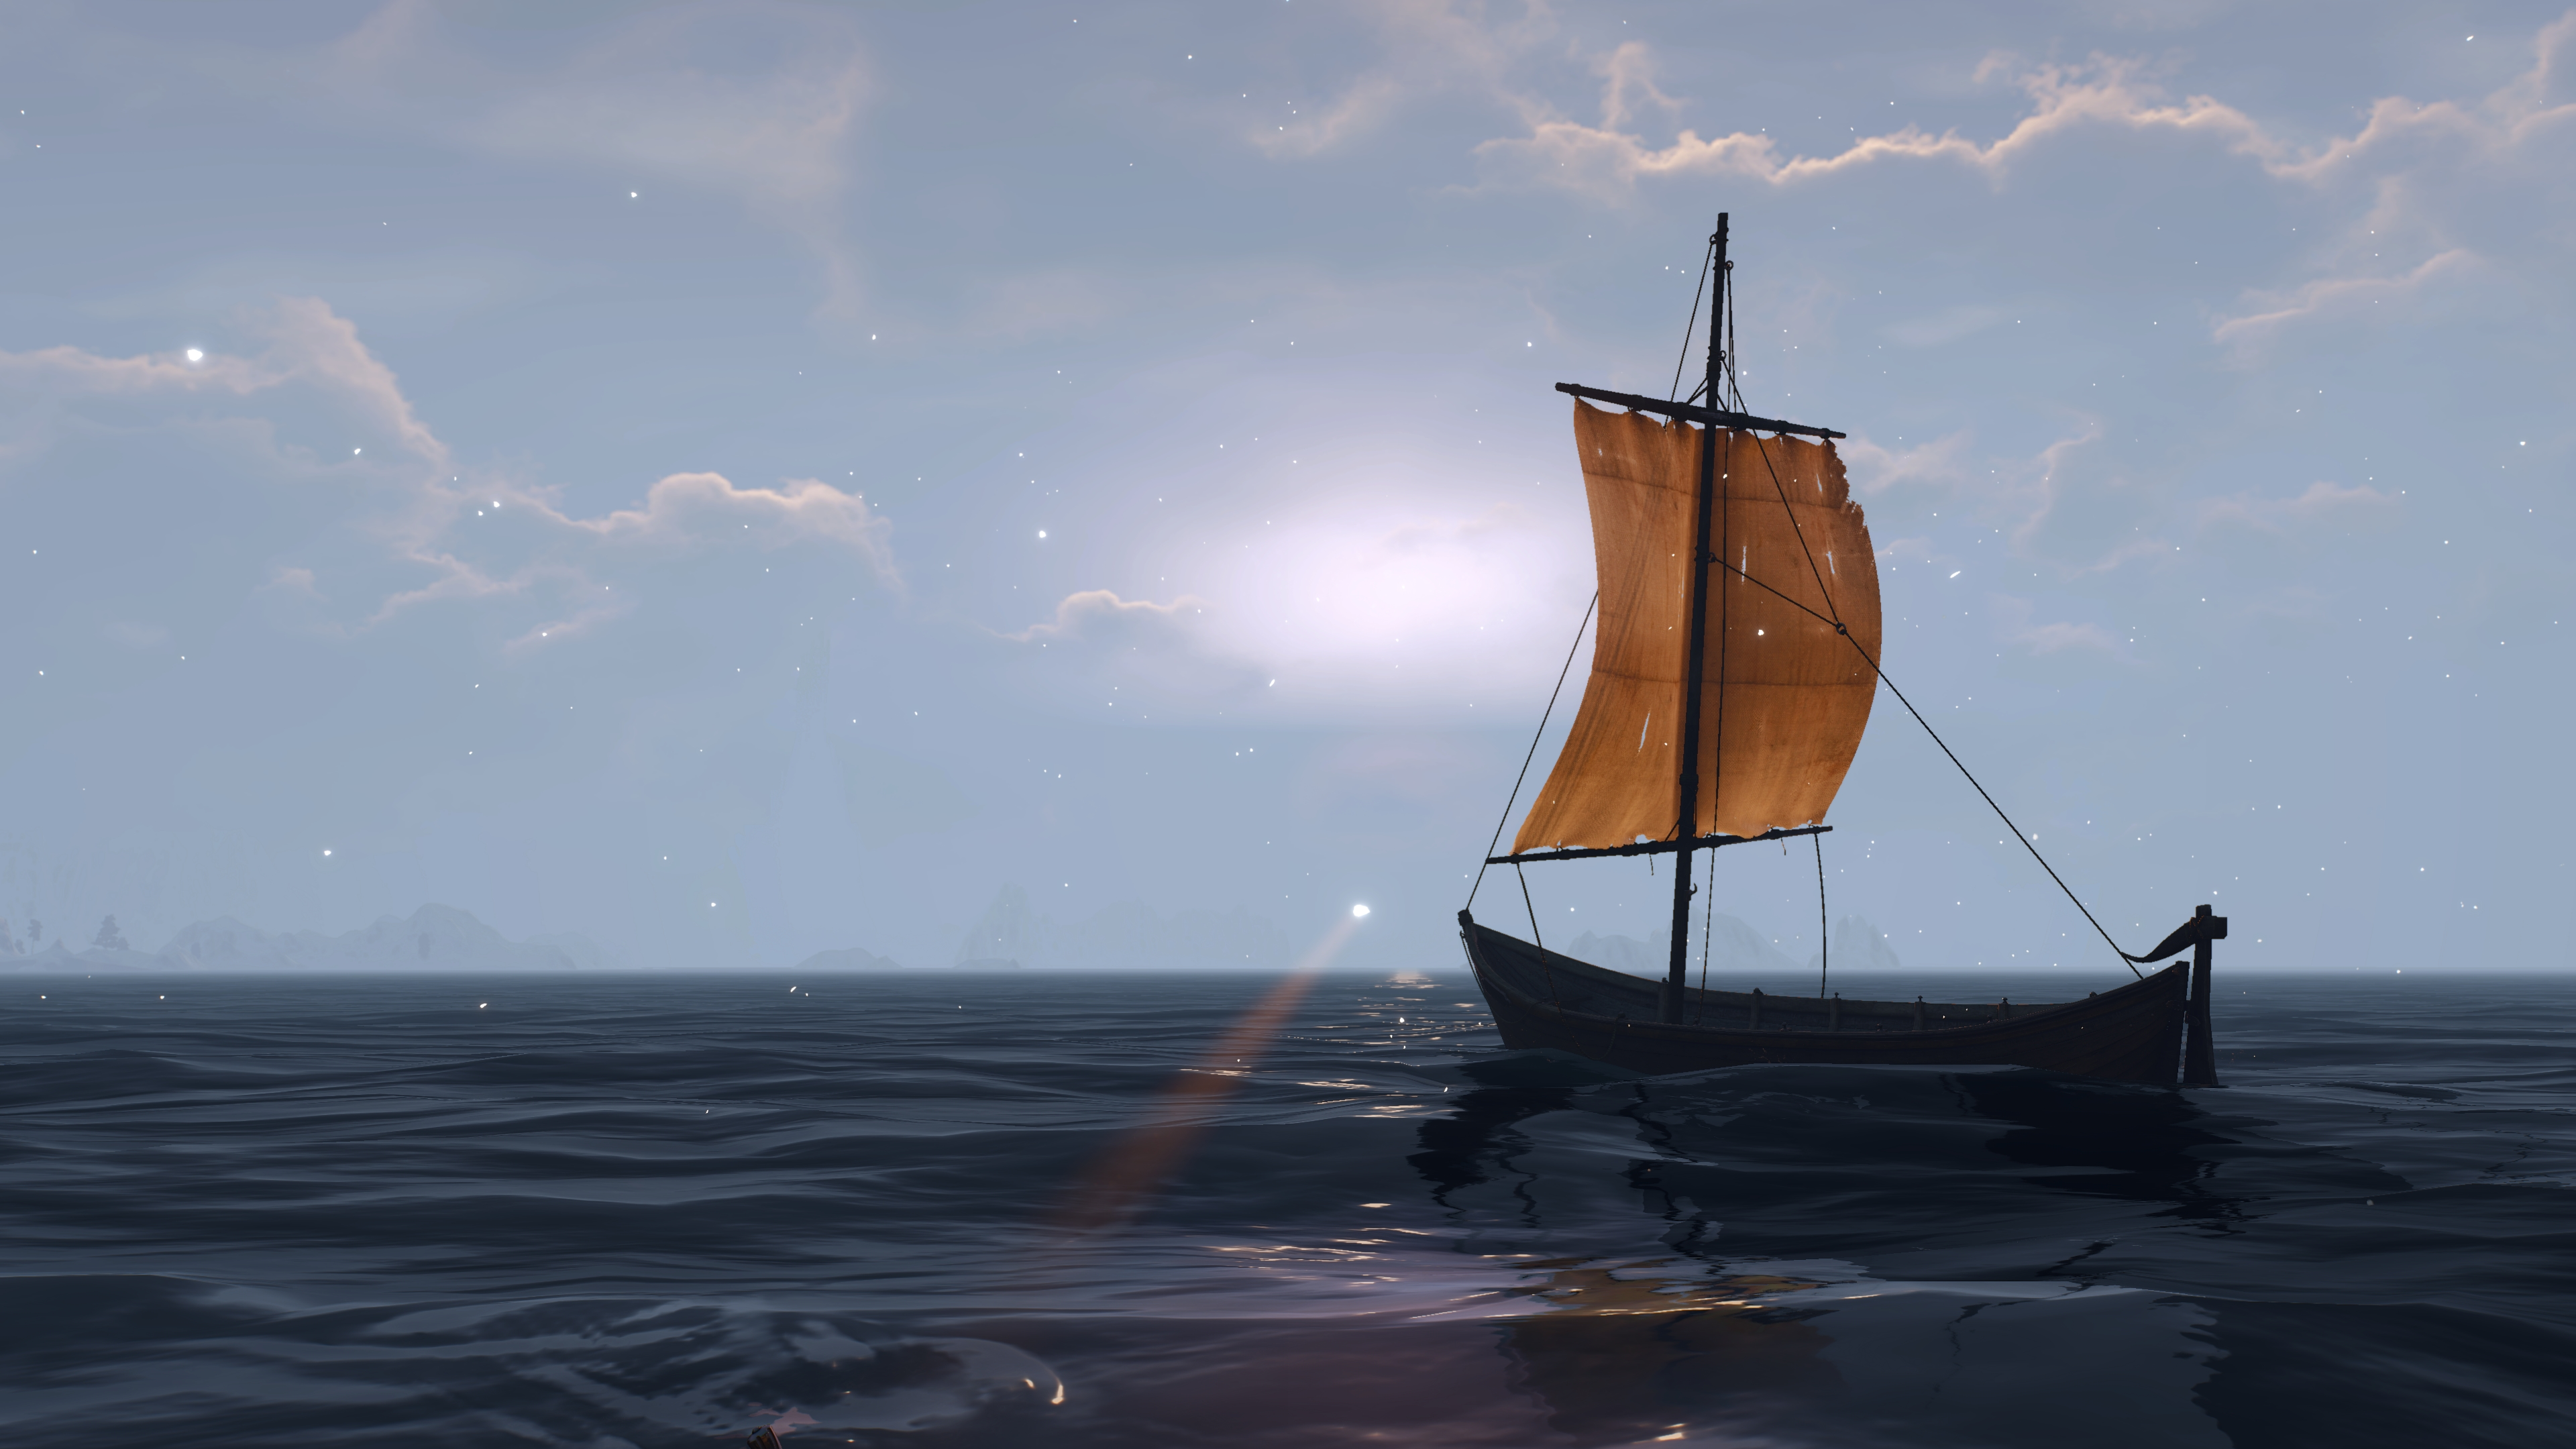
\includegraphics[width=0.95\textwidth]{./Examples/boat.jpg}
    \caption{A boat}
    \label{fig1: Boat}
\end{figure}

%%%%Works cited
\begin{workscited}

\bibent
Negr\'{o}n-Gonzales, Genevieve. ``Navigating `Illegality': Undocumented Youth \& Oppositional Consciousness.'' \textit{Children and Youth Services Review}, vol. 35, no. 8, 2013, pp. 1284-1290

\bibent
Spade, Dean. ``Solidarity Not Charity: Mutual Aid for Mobilization and Survival.'' \textit{Social Text}, 38.1, 2020, pp. 131-151


\end{workscited}


\end{flushleft}
\end{document}
